\documentclass{article}
\usepackage{amsmath}
\usepackage{titlesec}
\usepackage[utf8x]{inputenc}
\usepackage[margin=1.5in]{geometry}
\usepackage{enumerate}
\newtheorem{theorem}{Theorem}
\usepackage[dvipsnames]{xcolor}
\usepackage{pgfplots}
\pgfplotsset{compat=1.18}
\setlength{\parindent}{0cm}
\usepackage{graphics}
\usepackage{graphicx} % Required for including images
\usepackage{subcaption}
\usepackage{bigintcalc}
\usepackage{pythonhighlight} %for pythonkode \begin{python}   \end{python}
\usepackage{appendix}
\usepackage{arydshln}
\usepackage{physics}
\usepackage{booktabs} 
\usepackage{adjustbox}
\usepackage{mdframed}
\usepackage{relsize}
\usepackage{physics}
\usepackage[thinc]{esdiff}
\usepackage{esint}  %for lukket-linje-integral
\usepackage{xfrac} %for sfrac
\usepackage[colorlinks=true]{hyperref} %for linker, må ha med hypersetup
\usepackage[noabbrev, nameinlink]{cleveref} % to be loaded after hyperref
\usepackage{amssymb} %\mathbb{R} for reelle tall, \mathcal{B} for "matte"-font
\usepackage{listings} %for kode/lstlisting
\usepackage{verbatim}
\usepackage{graphicx,wrapfig,lipsum,caption} %for wrapping av bilder
\usepackage{mathtools} %for \abs{x}
\usepackage[english]{babel}
\usepackage{cancel}
\usepackage{mhchem} % for atom notasjon
\definecolor{codegreen}{rgb}{0,0.6,0}
\definecolor{codegray}{rgb}{0.5,0.5,0.5}
\definecolor{codepurple}{rgb}{0.58,0,0.82}
\definecolor{backcolour}{rgb}{0.95,0.95,0.92}
\lstdefinestyle{mystyle}{
    backgroundcolor=\color{backcolour},   
    commentstyle=\color{codegreen},
    keywordstyle=\color{magenta},
    numberstyle=\tiny\color{codegray},
    stringstyle=\color{codepurple},
    basicstyle=\ttfamily\footnotesize,
    breakatwhitespace=false,         
    breaklines=true,                 
    captionpos=b,                    
    keepspaces=true,                 
    numbers=left,                    
    numbersep=5pt,                  
    showspaces=false,                
    showstringspaces=false,
    showtabs=false,                  
    tabsize=2
}

\lstset{style=mystyle}
\author{Oskar Idland}
\title{test}
\date{}
\begin{document}
\maketitle
\tableofcontents
\newpage

\section{History}
\begin{itemize}
    \item 1896: Henri Becquerel discovered radioactivity
    \item 1898: Marie and Pierre Curie discovered radium and polonium
    \item 1903: Alphas charge to mass ratio
    \item 1909: Alphas are helium nuclei
    \item 1911: Rutherford discovers the nucleus
    \item 1913: Bohr model of the atom
    \item 1917: Rutherford discovers the proton
    \item 1930: Neutrinos were postulated 
    \item 1932: Chadwick discovers the neutron by shooting alpha particles at beryllium. 
    \item 1938: Discovery of nuclear fission
    \item 1956: Neutrinos were detected 
\end{itemize}

\subsection{Proton Discovery: The Rutherford Scattering Experiment}

Thomson's model of the atom was a positive sphere with electrons embedded in it. Rutherford wanted to test this model by shooting alpha particles at a thin gold foil surrounded by a detector foil. The alpha particles were shot from a radioactive source and when the alpha particles exited, they hit the foil and emitted light. 
\subsubsection{Conclusion}
\begin{itemize}
    \item Most alpha particles went straight through the foil. This implies the atom is mostly empty space.
    \item Some alpha particles were deflected by a small angle. This implies the positive charge is concentrated in a small volume.
    \item Sometimes the particles travel backwards. This implies the positive center has most of the mass of the atom.
\end{itemize}

\subsection{Discovery of the Neutron}
\begin{itemize}
    \item Shooting alpha particles on beryllium which is much lighter than gold. This 
\end{itemize}

\section{Nucleus}
\begin{itemize}
    \item Very dense. Carries all the mass. $2.7 ⋅ 10^{14}$ times denser than water.
    \item The atom is mostly empty space. If the nucleus was the size of a coin, the atom would be 2-3 km in radius. 
\end{itemize}
\subsection{Notation}
\begin{itemize}
    \item \textbf{Notation}: $_{Z}^{A}X_{N}$ 
    \item Isoto\textbf{p}e: Same \textbf{proton} number $Z$
    \item Isoto\textbf{n}e: Same \textbf{neutron} number $N$
    \item Isob\textbf{a}r: Same \textbf{atomic} mass number $A = Z + N$
\end{itemize}

\subsection{Nuclides}
\begin{itemize}
    \item 92 stable elements
    \item 280 stable isotopes
    \item 3000 unstable isotopes
    \item 6000 more predicted to exist
\end{itemize}
\subsubsection{Stable Numbers}
\begin{equation}
N = 2, 8, 20, 28, 50, 82, 126
\end{equation}
\begin{equation}
Z = 2, 8, 20, 28, 50, 82, \ldots     
\end{equation}
\section{Units and Dimensions in Nuclear Physics}
\subsection{Length}
The order of $10^{-15}$m = 1fm (fermi/femtometer) meter. This is the distance between nucleons.

\subsection{Time Scale}
\begin{itemize}
    \item $10^{-20}$s: Unbound, in the case of nuclear reactions and decays. 
    \item $10^{-9}$/$10^{-12}$s: lifetimes of excited nuclear states through gamma decays. 
    \item Minutes/hours/millions of years: Alpha and beta decays. 
\end{itemize}

\subsection{Energy}
MeV in nuclear physics. 
\begin{equation}
    1 \text{ MeV} = 1.6 \times 10^{-13} \text{J}. 
    \end{equation}
    \begin{equation}
        1 \text{eV} = 1.6 \times 10^{-19} \text{J}
        \end{equation}

\subsection{Mass}
u = unified atomic mass unit. 1 u is defined as 1/12 of the mass of an unbound $^{12}$C atom. Mass is equivalent with energy. Therefore:
\begin{equation}
u = 931.5 \text{ MeV} / c^2 = 1.66 \times 10^{-27} \text{kg}
\end{equation}
\begin{figure}[ht!]
    \centering
    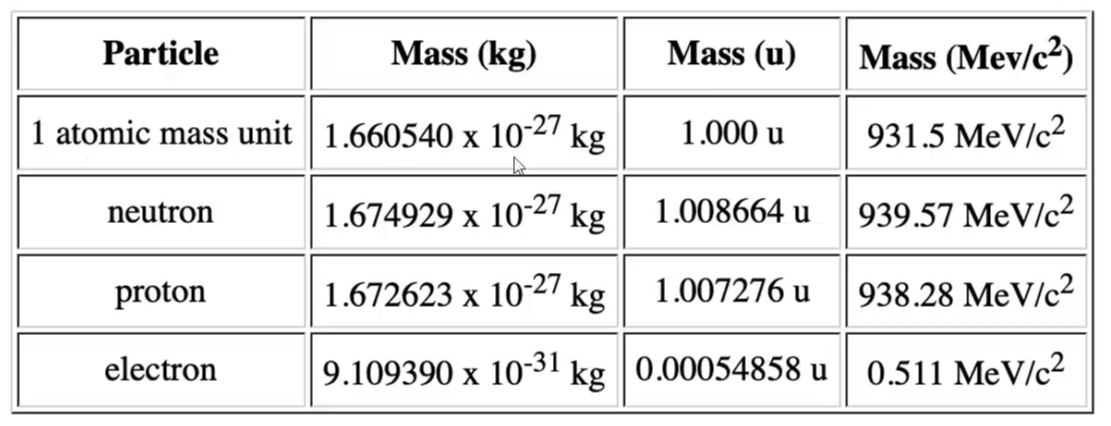
\includegraphics[width = \textwidth]{nucleon_mass_table.png}
    \caption{Table of the masses of the nucleons. $c^2 = 931.5$MeV/u. In reality, the mass of the proton is slightly less than the mass of the neutron. The proton is 2000 times more massive than the electron.}
    \label{fig: }
\end{figure}


\section{Nuclear Properties}
The parameters which describe the nucleus are. There are two types of nuclear properties: static and dynamic.
\begin{itemize}
    \item Static: Charge, Radius, mass, Binding energy, Angular momentum, Parity, Magnetic dipole moment, Electric quadrupole moments, Exited states and their energies. 
    \item Dynamic: Shape, Decay
\end{itemize}

\subsection{Connected Terms}
\begin{itemize}
    \item Charge/Charge Distribution: Protons. Found via electron scattering \cref{subsec: Nuclear Charge Distribution from Electron Scattering} by the Coulomb interaction. 
    \item Matter/Mass Distribution: Nucleons. Found via hadron scattering \cref{subsec: Nuclear Mass Distribution from Hadron Scattering}, alpha particles (Rutherford), protons and neutrons by using the strong force.
    \item Radius: Size of the nucleus (nucleons)
\end{itemize}

\subsection{Charge Distribution}
To probe the charge distribution of the nucleus, we use charged particles. We also need the following:
\begin{itemize}
    \item A beam of charged particles (often protons)
    \item Wavelength should be similar or smaller than the nucleus (about 10fm in diameter). 
    \item Electrons were popular in the 50's. 
    \item An energy of 100 Mev to 1 GeV is needed.
    \item Calculating the energy needed is done by using the de Broglie wavelength where $λ = h / p$ with $λ ≤ 10$fm. 
\end{itemize}

\subsection{Nuclear Charge Distribution from Electron Scattering}\label{subsec: Nuclear Charge Distribution from Electron Scattering}
\begin{itemize}
    \item Radius increases with mass number $A$
    \item The central nuclear charge density is nearly the same for all nuclei. Nucleons do not seem to concentrate near the center of the nucleus, but instead have a constant distribution along the surface. 
    \item The number of nucleons per unit volume is roughly constant:
    \begin{equation}
    \frac{A}{\frac{4}{3}πR^3} ≈ \text{const}
    \end{equation} 
    \item The radius of the nucleus is proportional to $A^{1/3}$. 
    \begin{equation}
    R = R_0A^{1/3} \quad , \quad  R_0 ≈ 1.2 \text{ fm}
    \end{equation}
\end{itemize}

\subsection{Nuclear Size}
We can find the radius of a nucleus by using the scattering angle of the local minimum of the Rutherford cross-section, see \cref{fig: electron_scattering_angles}. The diffraction pattern is not exactly that of a circular disk, as the nucleus does not have a well-defined surface.
\begin{figure}[ht!]
\centering
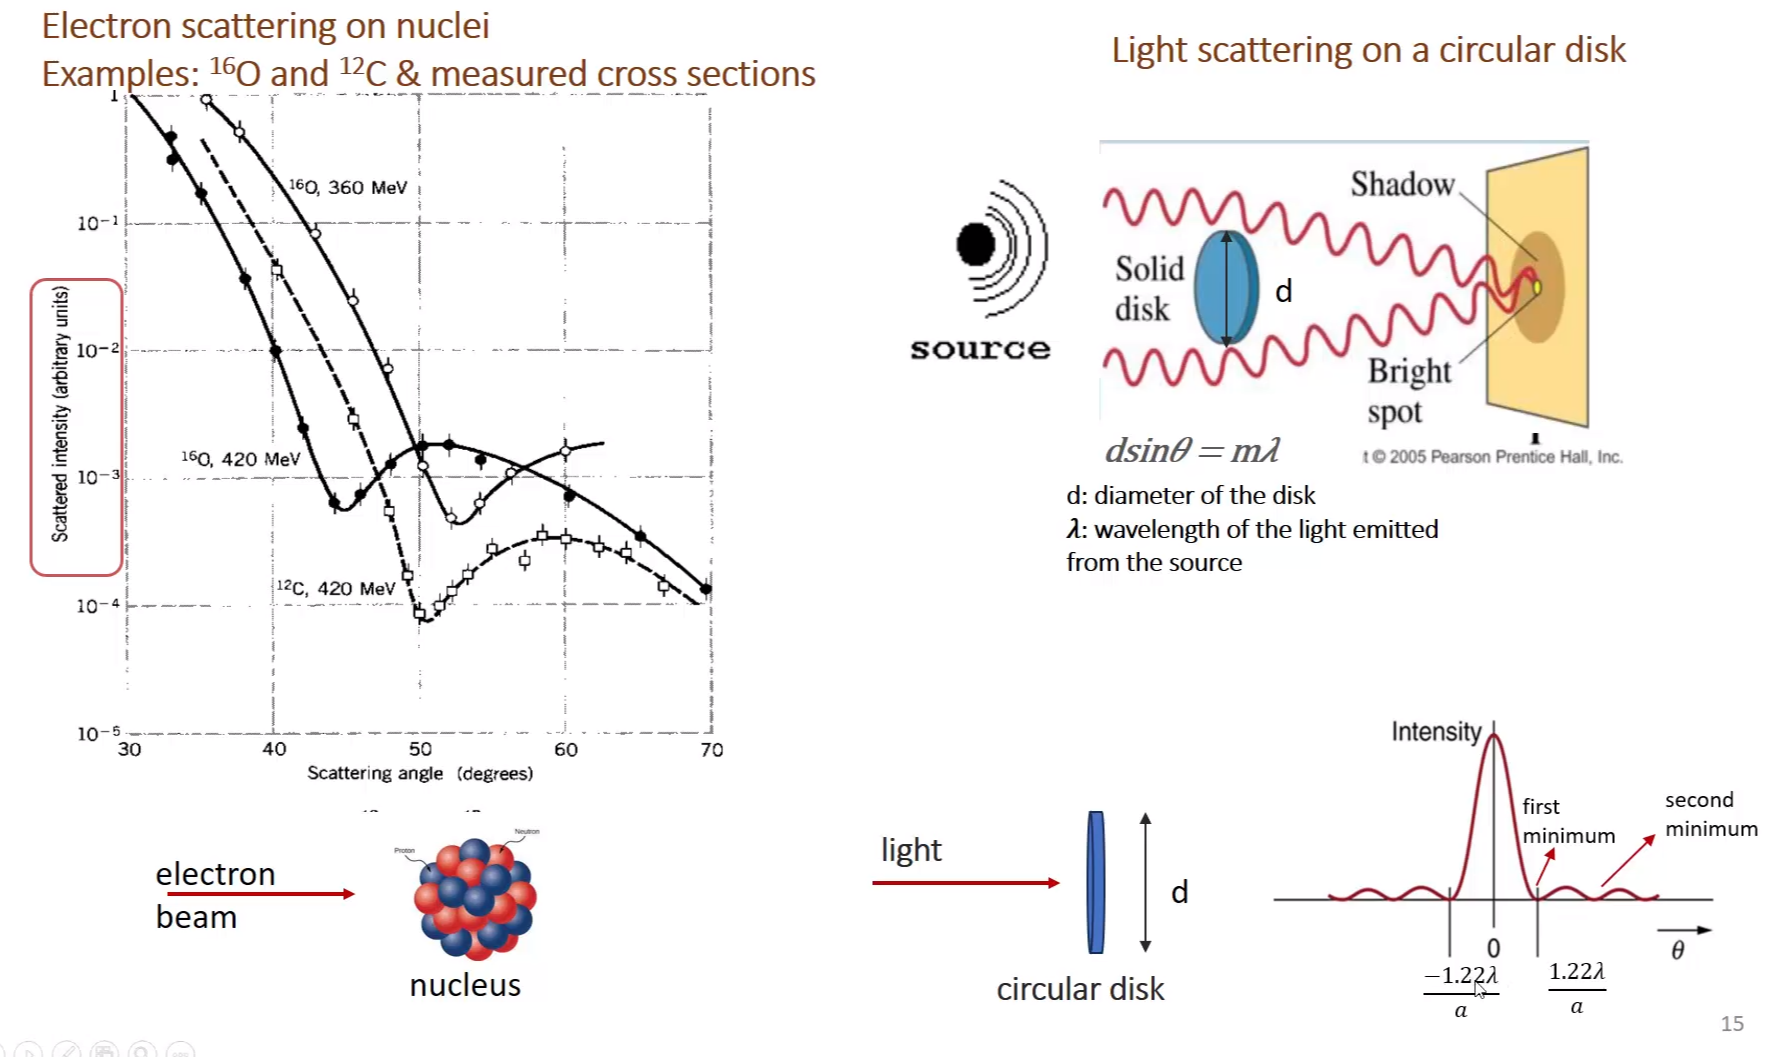
\includegraphics[width = \textwidth]{electron_scattering_angles.png}
\caption{Example of the local minimum of the Rutherford cross-section. The angle is used to calculate the radius of the nucleus.}
\label{fig: electron_scattering_angles}
\end{figure}
\begin{equation}
\sin θ = \frac{1.22λ}{d} ⇒ R = \frac{d}{2} = \frac{1.22λ}{2\sin θ}
\end{equation}
This is only a rough estimate as the angle is calculated in two dimensions, instead of three. 


\subsection{Nuclear Mass Distribution from Hadron Scattering}\label{subsec: Nuclear Mass Distribution from Hadron Scattering}
\begin{itemize}
    \item Electrons only mostly interact with protons. We therefore use hadrons to study the mass distribution of the nucleus.
    \item The radius is proportional to the nuclear rather than the Coulomb force. 
    \item The Rutherford experiment showed that the nucleus is a point-like object.
\end{itemize}

\subsubsection{Fixed Angle of Observation with Changing Energy}
\begin{itemize}
    \item At low energies the alpha particles and the $^{208}$Pb nucleus interact with the Coulomb interacting as with Rutherford scattering.
    \item With increasing energy, the repulsion from the Coulomb force is overcome, and the strong force becomes the dominant force. The Rutherford formula no longer holds. 
    \item The alpha particles became absorbed by the nucleus and only a small fraction is scattered. 
    \item When energy is high enough, we get the diffraction pattern.
\end{itemize}

\subsection{Conclusion from Charge Radius Experiments}
\begin{itemize}
    \item The charge and mass radii of nuclei is nearly equal to within about $0.1$fm. 
    \item Both show the same $A^{1/3}$ dependence with $R_0 = 1.2$fm. 
    \item As heavy nuclei have about 50 \% more neutrons than protons, we might expect the neutron distribution to be more extended than the proton distribution. This is not the case as the neutrons pulls inwards, and the protons push outwards, until they are mixed such that the radius is the same. 
\end{itemize}



\subsection{Nuclear Mass}
\subsection{Deflection Spectrometer}
\begin{figure}[ht!]
\centering
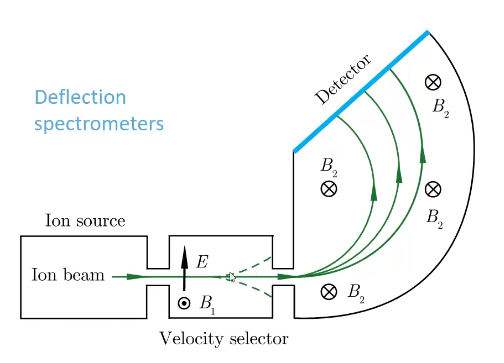
\includegraphics[width = .5\textwidth]{deflection_spectrometer.png}
\caption{Experimental setup for measuring the mass of a particle.}
\label{fig: deflection_spectrometer}
\end{figure}

\begin{itemize}
    \item Shooting a ray of charge particles affected by a magnetic field and measuring the deflection we can calculate its mass. 
    \item To measure an entire particle they must be ionized. The electrons carry so little mass that they are neglected.
    \item After ionization, the particles travel through an electric and magnetic field. 
    \item Only the particles with the right velocity will pass through the fields and be subjected to the new magnetic field. 
    \item The new field will deflect the particles according to their $m / q$ value. 
\end{itemize}
\subsubsection{Calculating the Mass}
\begin{equation}
F_{B} = q \vec{v} × \vec{B} 
\end{equation}
The field and velocity are perpendicular.
\begin{equation}
F_{B} = qvB
\end{equation}
\begin{equation}
F_E = F_B ⇒ qE = qvB ⇒ v = \frac{E}{B_1}
\end{equation}
$B_1$ is the first magnetic field as seen in \cref{fig: deflection_spectrometer}. The force from the magnetic field centripetal force. 
\begin{equation}
F_B = \frac{mv^2}{r} = qvB_2
\end{equation}
\begin{equation}
\frac{mv}{r} = qB_2
\end{equation}
\begin{equation}  
\frac{m}{q} = \frac{B_2ρ}{v}
\end{equation}
The radius of the circle is given by $r = ρ$. Setting $B_1 = B_2$ gives the following for the mass.
\begin{equation}
m = \frac{B_1 B_2 ρ}{E} = \frac{B^2 ρq}{E}
\end{equation}
where $q$ is the charge of the particle.

\paragraph{Accuracy}
\begin{itemize}
    \item These measurements are very important for mass models used in other parts of physics. 
    \item The accuracy is about $Δm / m = 10^{6-}$, but that is not enough. 
    \item The mass doublet technique gives a precision of $10^{-8}$ / $10^{-9}$
\end{itemize}






\section{Binding Energy}
\subsection{Formulas and Definitions}
\begin{itemize}
    \item Binding Energy: The energy required to keep the nucleus together. The mass of the nucleus is not equal to the sum of its parts. The mass of the individual nucleons is higher than the mass of the nucleus. The difference is the binding energy.
    \begin{equation}
    Zm_p + Nm_n - M_{\text{Nucleus}} = \text{Binding Energy}  \quad ⇒ \quad Zm_p + Nm_n > M_{\text{Nucleus}}
    \end{equation}
\end{itemize}

\subsection{Mass of the Nucleus}
The total mass of the atom is the mass of the nucleus and electrons, minus the binding energy of the electrons. 
\begin{equation}
M_{\text{Atom}} = M_{\text{Nucleus}} + Zm_e - \underbrace{∑_{i=1}^{Z} B_i / c^2}_{\text{Often negligible}}
\end{equation}

\begin{equation}
M_{\text{Atom}} = M_{\text{Nucleus}} + Zm_e
\end{equation}

$M$ usually refers to the mass of the entire atom, and so the subscript "Atom" is often omitted. We usually write the atom using the following notation:
\begin{equation}
M\left(_{Z}^{A}X_{N}\right) = M_{\text{Nucleus}} \left(_{Z}^{A}X_{N}\right) + Zm_e
\end{equation}
Multiplying by $c^2$ we get the mass in energy units ($E = mc^2$):
\begin{equation}
M_{\text{Nucleus}}\left(_{Z}^{A}X_{N}\right) = M\left(_{Z}^{A}X_{N}\right) - Zm_ec^2
\end{equation}
\begin{equation}
\underline{\underline{M_{\text{Nucleus}}\left(_{Z}^{A}X_{N}\right)c^2 = M\left(_{Z}^{A}X_{N}\right)c^2 - Zm_e c^2 
}}
\end{equation}
\subsection{Nuclear Binding Energy (B.E.)}
This energy is very small compared to the mass energy of the nucleus. We can derive this from the mass of the nucleus. 
\begin{align}
    B.E. &= \left(Zm_{p} + Nm_{n} - M_{N}\left(_{Z}^{A}X_{N}\right)\right) c^2 \\
    &= \left(Zm_{p} + Nm_{n} - \left(M\left(_{Z}^{A}X_{N}\right) - Zm_e\right)\right) c^2 \\ 
    &= \left(Z(\underbrace{m_{p} + m_e}_{\text{Hydrogen}}) + Nm_{n} - M\left(_{Z}^{A}X_{N}\right)\right) c^2 \\ \\
   B.E. &= \underline{\underline{\left(Zm\left(^{1}H\right) + Nm_{n} - M\left(_{Z}^{A}X_{N}\right)\right) c^2}}
\end{align}
As the units so far has been energy $(mc^2)$ we can switch to MeV. 
\begin{equation}
B.E. = \left[mc^2\right] = \left[uc^2\right] = u931.5\text{MeV /}u \quad ⇒ \quad c^2 = 931.5 \text{MeV/u}
\end{equation}
\begin{equation}\label{eq: binding_energy}
B.E. = \underline{\underline{\left(Zm\left(^{1}H\right) + Nm_{n} - M\left(_{Z}^{A}X_{N}\right)\right) 931.5 \text{MeV/u}}}
\end{equation}

\subsubsection\protect{Example: Helium $_{2}^{4}H_{2}$}
We use the formula for binding energy from \cref{eq: binding_energy} to calculate the binding energy of the hydrogen atom $_{2}^{4}He_{2}$.
\begin{align}
B.E. &= \left(2m_p + 2m_n - M\left(_{2}^{4}He_{2}\right)\right) 931.5 \text{MeV/u} \\
&= \left(2 ⋅ 1.007825u + 2 ⋅ 1.008664u - 4.002603u\right) ⋅ 931.5 \text{MeV/u} \\
&= \underline{\underline{0.0304 ⋅  931.5 \text{ MeV} = 28.3 \text{ MeV}}}\label{eq: helium_binding_energy}
\end{align}
The ratio between the binding energy and the rest mass of the nucleus is very small. Using the binding energy from \cref{eq: helium_binding_energy} and the mass of the helium nucleus, we can calculate the ratio:
\begin{equation}
\frac{28.3}{3728} = 0.75\%
\end{equation}
\subsection{Nuclear Separation Energy}
The energy required to separate a proton $S_{p}$ or a neutron $S_{n}$ from the nucleus.
\subsubsection{Neutron Separation Energy}\label{sssec: neutron_separation_energy}
It requires lower energy to remove a neutron from a nucleus with an odd number of neutrons. This is because one is unpaired. 
\begin{equation}
S_n = \left(M\left(_{Z}^{A-1}X_{N-1}\right) - M(_{Z}^{A}X_{N} + m_n)\right)c^2
\end{equation}
This can also be expressed using binding energies as mass and energy are equivalent through $E = mc^2$:
\begin{equation}
S_n = B\left(_{Z}^{A}X_{N}\right) - B\left(_{Z}^{A-1}X_{N-1}\right)
\end{equation}

\subsubsection{Proton Separation Energy}
Using the same logic as for the neutron separation energy \cref{sssec: neutron_separation_energy}, we can express the proton separation energy through the binding energies. It's important to keep in mind that after loosing a proton, the element changes.
\begin{equation}
S_p= \left(M\left(_{Z-1}^{A-1}Y_{N}\right) - M(_{Z}^{A}X_{N} + \underbrace{m_p + m_n}_{_{1}^{1}H_{}})\right)c^2
\end{equation}
\begin{equation}
S_p = B\left(_{Z}^{A}X_{N}\right) - B\left(_{Z-1}^{A-1}Y_{N}\right)
\end{equation}

% \subsection{Average Binding Energy}
\begin{itemize}
    \item Except for very light nuclei, the binding energy per nucleon is linear. It's almost constant at around 8 MeV/nucleon.
    \item The highest binding energy per nucleon is around $A = 60$ with the highest binding energy per nucleon at $^{56}\text{Fe}$. 
    \item When going from heavier elements towards iron we get nuclear fission
    \item When going from lighter elements towards iron we get nuclear fusion
\end{itemize}

\begin{figure}[h!]
\centering
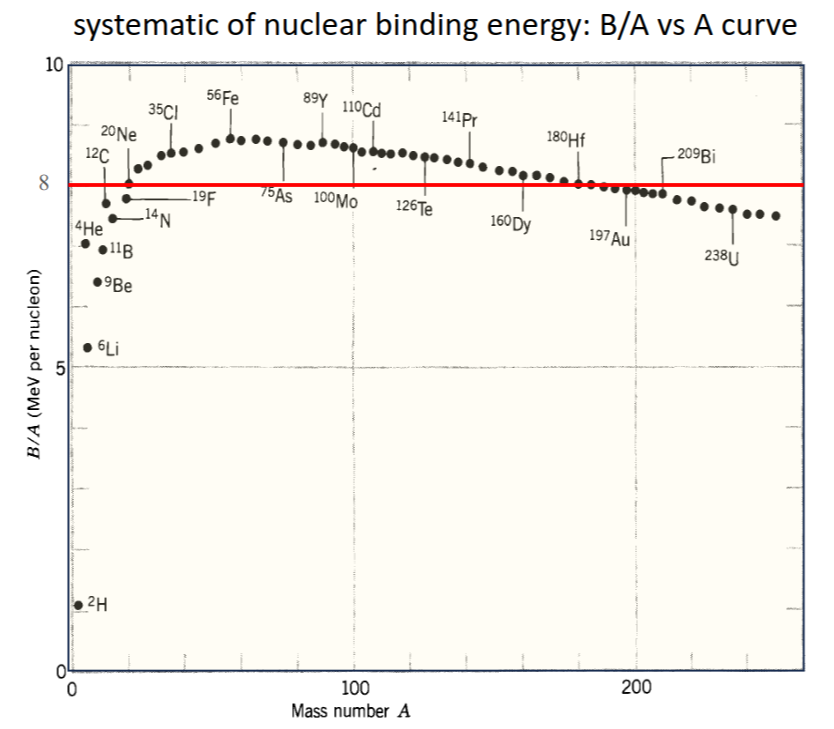
\includegraphics[width = .75\textwidth]{BE_per_nucleon.png}
\caption{}
\label{fig: BE_per_nucleon}
\end{figure}

\subsection{Semi-Empirical Mass Formula}
\begin{itemize}
    \item Sets out to explain the binding energies of nuclei.
    \item It is semi-empirical as the five of its constant are found by experiment.
    \item Tries to recreate the binding energy per nucleus graph in \cref{fig: BE_per_nucleon} by using the \textit{liquid drop model}.
\end{itemize}

\begin{equation}\label{eq: semi_empirical_mass_formula}
B = a_vA - a_sA^{2 / 3} - a_c\frac{Z(Z-1)}{A^{1 / 3}} - a_{\text{asym}}\frac{(A-2Z)^2}{A} + δ
\end{equation}
\subsubsection{Explanation of the Terms in the Semi-Empirical Mass Formula}\label{sssec: Explenation of the Terms in the Semi-Empirical Mass Formula}
\begin{itemize}
    \item $\mathbf{a_vA}$: \textbf{Volume term}. The binding energy is proportional to the volume of the nucleus approximated to a sphere $\left(V = 4πR^3/3\right)$. This dominates the binding energy for large nuclei. 
    \begin{equation}
    a_v ≈ 15.8 \text{ MeV}
    \end{equation}
    The linear dependence of the binding energy on the number of nucleons tells us that the strong force is short range as each nucleon only interacts with its nearest neighbors. 
    \item $\mathbf{a_sA^{2 / 3}}$: \textbf{Surface term}. The volume term is not quite accurate as the nucleons on the surface have fewer neighbors. This term corrects for that. The binding energy is proportional to $πR^2$
    \begin{equation}
    a_s ≈ 16.8 \text{ MeV}
    \end{equation} 
    \item $\mathbf{a_cZ(Z-1)A^{-1 / 3}}$: \textbf{Coulomb term}. The binding energy is reduced by the repulsion between the protons. It is therefore detracted. The Coulomb force is long range and is therefore proportional to $Z(Z-1)$ as all protons interact. 
    \begin{equation}
    a_c ≈ 0.72 \text{ MeV}
    \end{equation}
    \item $\mathbf{a_{\text{asym}}(A-2Z)^2A^{-1}}$: \textbf{Asymmetry term}. Stable nuclei have a balance between protons and neutrons. As the ratio of protons to neutrons deviate from 1, the nuclei becomes less stable (lower binding energy). This inhibits Hydrogen or Helium atoms with many neutrons. It is caused by the Pauli exclusion principle as nucleons are fermions and therefore can not occupy the same state at once. 
    \begin{equation}
    a_{\text{asym}} ≈ 23 \text{ MeV}
    \end{equation}
    Heavier nuclei must have more neutrons to fight the Coulomb repulsion. The term gets relatively small as the number of nucleons increases. 
    \item $\mathbf{δ}$: \textbf{Pairing term}. This term is not included in the original formula, but is added to account for the fact that nuclei with an even number of protons and neutrons are more stable. This is because the nucleons in the same space-state can be coupled to have a total spin of 0. They are therefore closer together and therefore more tightly bound with a higher binding energy. This is called even-even nuclei. 
    \begin{equation}
    δ =  \begin{cases}
        +a_pS^{-3 / 4}, &\text{ if even(N)-even(Z)}\\
        0, &\text{ if odd(A)}\\
        -a_pS^{-3 / 4}, &\text{ if odd(N)-odd(Z)}\\
    \end{cases} 
    \end{equation}
    \begin{equation}
    a_p ≈ 34 \text{ MeV}
    \end{equation}
\end{itemize}
\subsubsection{SEMF Conclusion}
\begin{itemize}
    \item The semi-empirical mass formula was a first attempt at understanding how binding energy works. 
    \item It is semi-empirical as the constants are found by experiment. 
    \item A negative binding energy means the nucleus is not bound and is therefore not stable.
\end{itemize}
\begin{equation}
B = \underbrace{a_vA - a_sA^{2 / 3} - a_cZ(Z-1)A^{-1 / 3}}_{\text{Liquid-drop model for energy calculations}} - \underbrace{a_{\text{asym}}(A-2Z)^2A^{-1} + δ}_{\text{Interactions between nucleons}}
\end{equation}
\begin{figure}[h!]
\centering
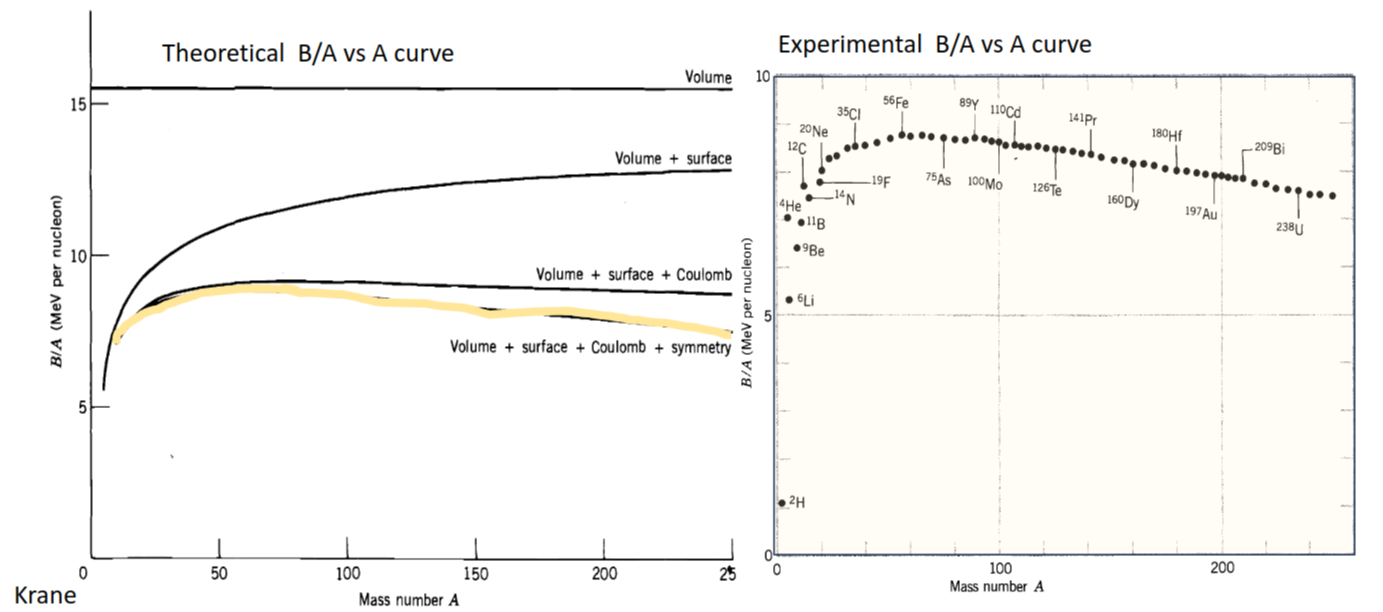
\includegraphics[width = \textwidth]{SEMF_term_addition.png}
\caption{Plot of how the different terms in the semi-empirical mass formula \cref{eq: semi_empirical_mass_formula} gets us closer to the experimental values}
\label{fig: SEMF_term_addition}
\end{figure}



\subsection{Mass Parabolas of Isobars}
Isobars have the same number of nucleons (A).
\begin{align}
M(A,Z) &= Z(\overbrace{m_p + m_e}^{M(_{}^{1}H_{})}) + (\underbrace{A-Z}_{\text{neut. num.}})m_n - B(A,Z) /c^2 \\
B(A,Z) &= a_vA - a_sA^{2 / 3} - a_c\frac{Z(Z-1)}{A^{1 / 3}} - a_a\frac{(A-2Z)^2}{A} + \delta(A,Z)
\end{align}
\subsubsection{Finding the Minimum of the Mass Parabola}
As the parabola is mass $M$ as a function of $Z$, we can find the minimum by taking the derivative with respect to $Z$ and setting it equal to zero.
\begin{align}
\frac{∂ M}{∂ Z} &= 0 \\
Z_{\text{min}} &= \frac{(m_n - m_p - m_e)+a_cA^{-1 / 3} + 4a_{\text{sym}}}{2a_{c} A^{-1 / 3} + 8a_{\text{sym}}A^{-1}}
\end{align}
We can approximate this as the following:
\begin{equation}
Z_{\text{min}} ≈ \frac{A}{2} \frac{1}{1 + \frac{1}{4}A^{2/3}a_c / a_{\text{sym}}} \quad , \quad  a_{\text{sym}} ≈ 23 \text{ MeV} \ , \ a_c ≈ 0.72 \text{ MeV}
\end{equation}

\paragraph{Example: A = 10}
This is stable for smaller nuclei. 
\begin{equation}
Z_{\text{min}} ≈ 5 \quad \text{ and } \quad  \frac{Z_{\text{min}}}{A} ≈ 0.5
\end{equation}

\paragraph{Example: A = 200}
A lower ratio is stable for larger nuclei.
\begin{equation}
Z_{\text{min}} ≈ 79 \quad \text{ and } \quad  \frac{Z_{\text{min}}}{A} ≈ 0.4
\end{equation}

\subsubsection{Valley of (beta) stability}
\begin{itemize}
    \item As can be seen in \cref{fig: valley_beta_stability}, we have two parabolas for $A = 128$ as it can be odd-odd or even-even. Higher binding energy is more stable.
    \item The even-even isobar is more stable as explained in \cref{sssec: Explenation of the Terms in the Semi-Empirical Mass Formula}, because the nucleons can pair up in the same space-state with opposite spins and therefore be closer to each other and thus more stable.
    \item Only the atom in the bottom of the valley is stable. The others are prompt to beta decay downwards. 
    \item Double beta decay can happen with even numbers of nucleons as can be seen for $A = 128$ with $Z = 52$, as $Z = 53$ has higher energy, and it is therefore forced to decay all the way up to $Z = 54$. 
\end{itemize}
\begin{figure}[h!]
\centering
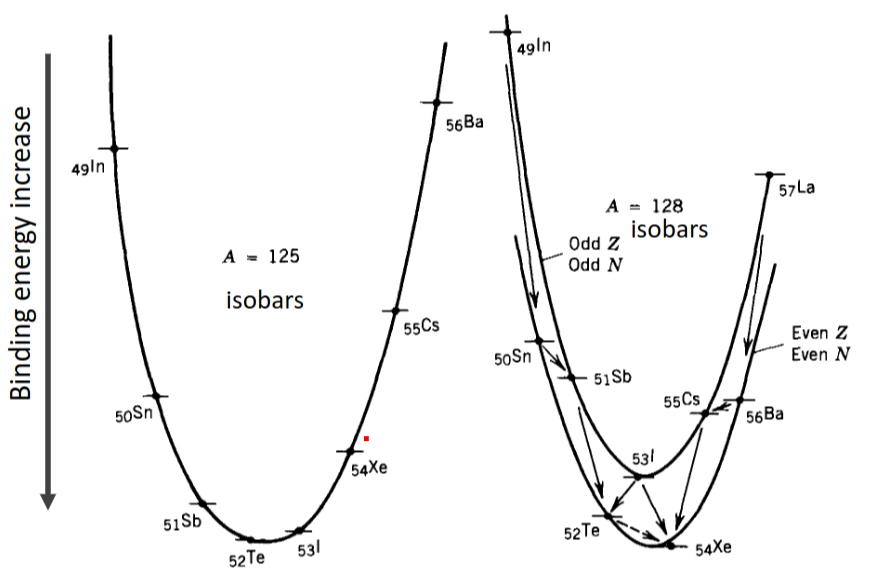
\includegraphics[width = .6\textwidth]{valley_beta_stability.png}
\caption{Valley of (beta) stability for different isobars with $A = 125$ and $A = 128$. The higher the binding energy, the more stable the isobar.}
\label{fig: valley_beta_stability}
\end{figure}

\paragraph{Beta Decay}
\begin{itemize}
    \item $β+$: Proton rich nuclei decay by converting a proton into a neutron, a positron and a neutrino. 
    \item $β-$: Neutron rich nuclei decay by converting a neutron into a proton, an electron and an antineutrino.
\end{itemize}
\begin{figure}[h!]
\centering
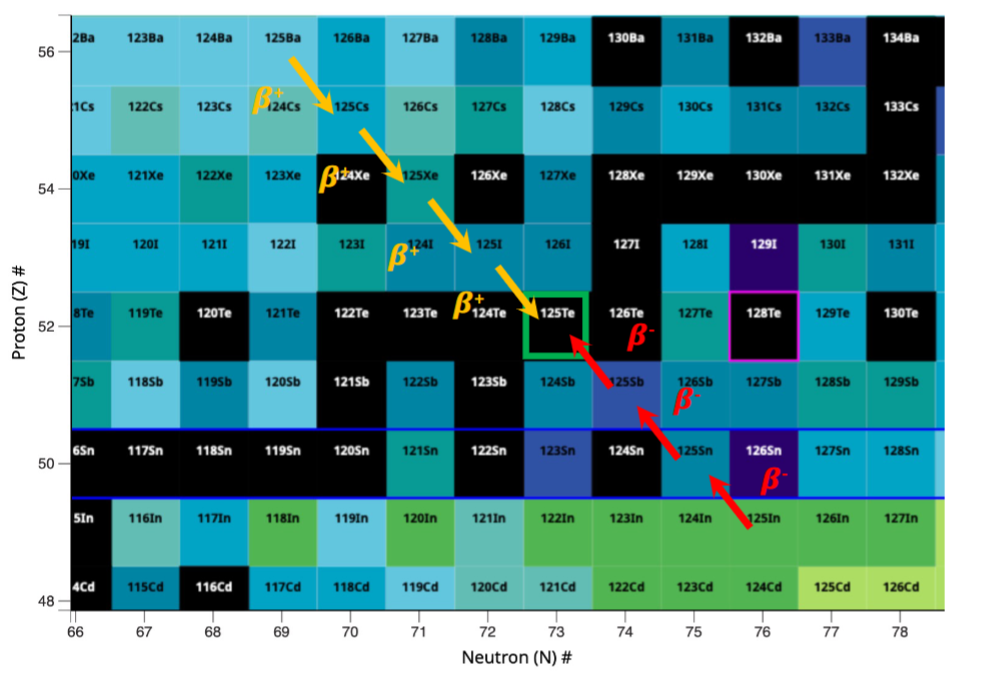
\includegraphics[width = \textwidth]{bet_decay_chart.png}
\caption{Chart showing different elements and their decays.}
\label{fig: bet_decay_chart}
\end{figure}


\section{Angular Momentum \& Parity}
\subsection{Angular Momentum of the Nucleus}
\begin{itemize}
    \item Total angular momentum $j = l + s$ is the sum of the orbital angular momentum $l$ and the spin $s$. 
    \item Both $l$ and $s$ are quantized, and the total angular momentum $j$ is also quantized.
    \item Nucleons are fermions and therefore spin half particles. 
    \item Fermions can't rotate, but still have spin $s$. There is no classical analogy for this. $l$ is the orbital angular momentum and is just like the classical angular momentum.
\end{itemize}
\subsubsection{Orbital Angular Momentum}
Angular momentum is a vector and thus has both magnitude and direction. As the values are quantized we use the quantum numbers $l$, $s$ and $j$ to describe the magnitude and direction. 
\begin{itemize}
    \item $l$ is the orbital angular momentum and can take the values $0, 1, 2, 3, \ldots$.
    \item Magnitude: 
    \begin{align}
    l &= \sqrt{l(l+1)}ℏ \\
    l_z &= m_lℏ \quad , \quad m_l ∈ \{-l, -l+1, \ldots, l-1, l\} 
    \end{align} 
    \item Direction \cref{fig: angular_momentum_sphere}:
    \begin{figure}[h!]
        \centering
        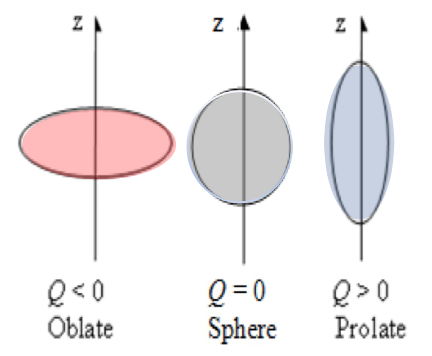
\includegraphics[width = .75\textwidth]{angular_momentum_sphere.png}
        \caption{Orbital angular momentum vector visualized on a sphere.}
        \label{fig: angular_momentum_sphere}
    \end{figure}
\end{itemize}    

\subsubsection{Spin}
\begin{itemize}
    \item Spin is a property of particles and is not related to the motion of the particle. 
    \item Spin is quantized and can take the values $s = \frac{1}{2}$ or $s = -\frac{1}{2}$.
    \item Magnitude: 
    \begin{align}
    s &= \sqrt{s(s+1)}ℏ \\
    s_z &= m_sℏ \quad , \quad m_s ∈ \{-s, -s+1, \ldots, s-1, s\} 
    \end{align} 
    \item As the spin $s$ can only be $1 / 2$, the magnetic quantum number $m_s$ can only be $\pm 1 / 2$
    \item Direction \cref{fig: spin_direction}: There is no classical analogy for direction, but if in a magnetic field, the spin will align with or against the field 
    \begin{figure}[h!]
    \centering
    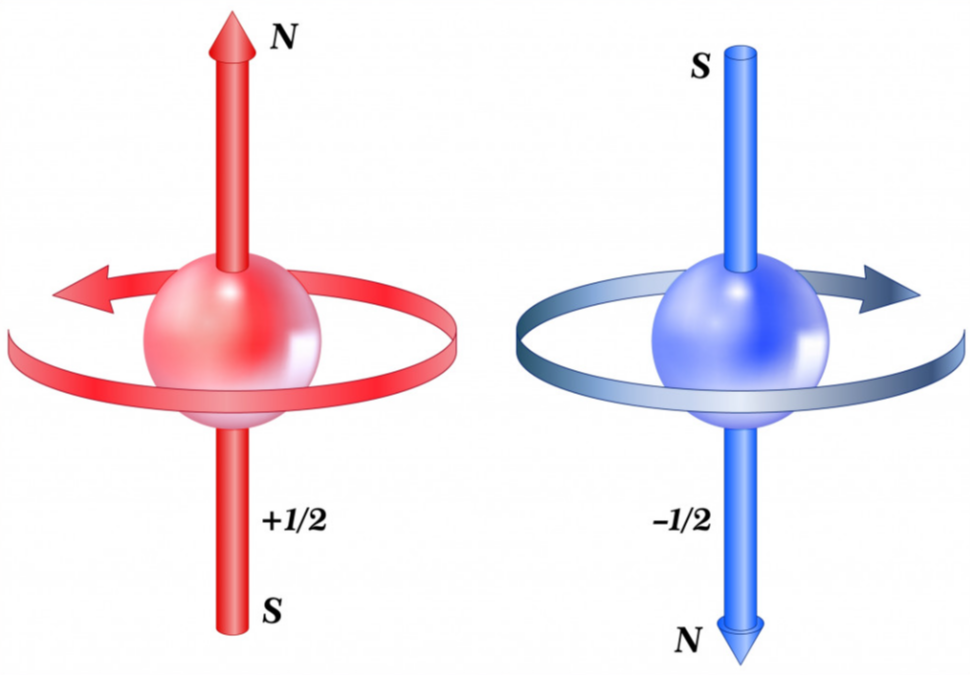
\includegraphics[width = .75\textwidth]{spin_direction.png}
    \caption{Visual representation of the spin of a nucleon in a magnetic field.}
    \label{fig: spin_direction}
    \end{figure}
\end{itemize}
\newpage
\subsubsection{Total Angular Momentum}
\begin{itemize}
    \item The total angular momentum $j$ is the sum of the orbital angular momentum $l$ and the spin $s$.
    \item Magnitude: 
    \begin{align}
    j &= \sqrt{j(j+1)}ℏ \\
    j_z &= m_jℏ \quad , \quad m_j ∈ \{-j, -j+1, \ldots, j-1, j\} \\
    m_j &= m_l + m_s = m_l ± \frac{1}{2}
    \end{align}
    \item Direction \cref{fig: total_angular_momentum_visualized}:
    \begin{figure}[h!]
    \centering
    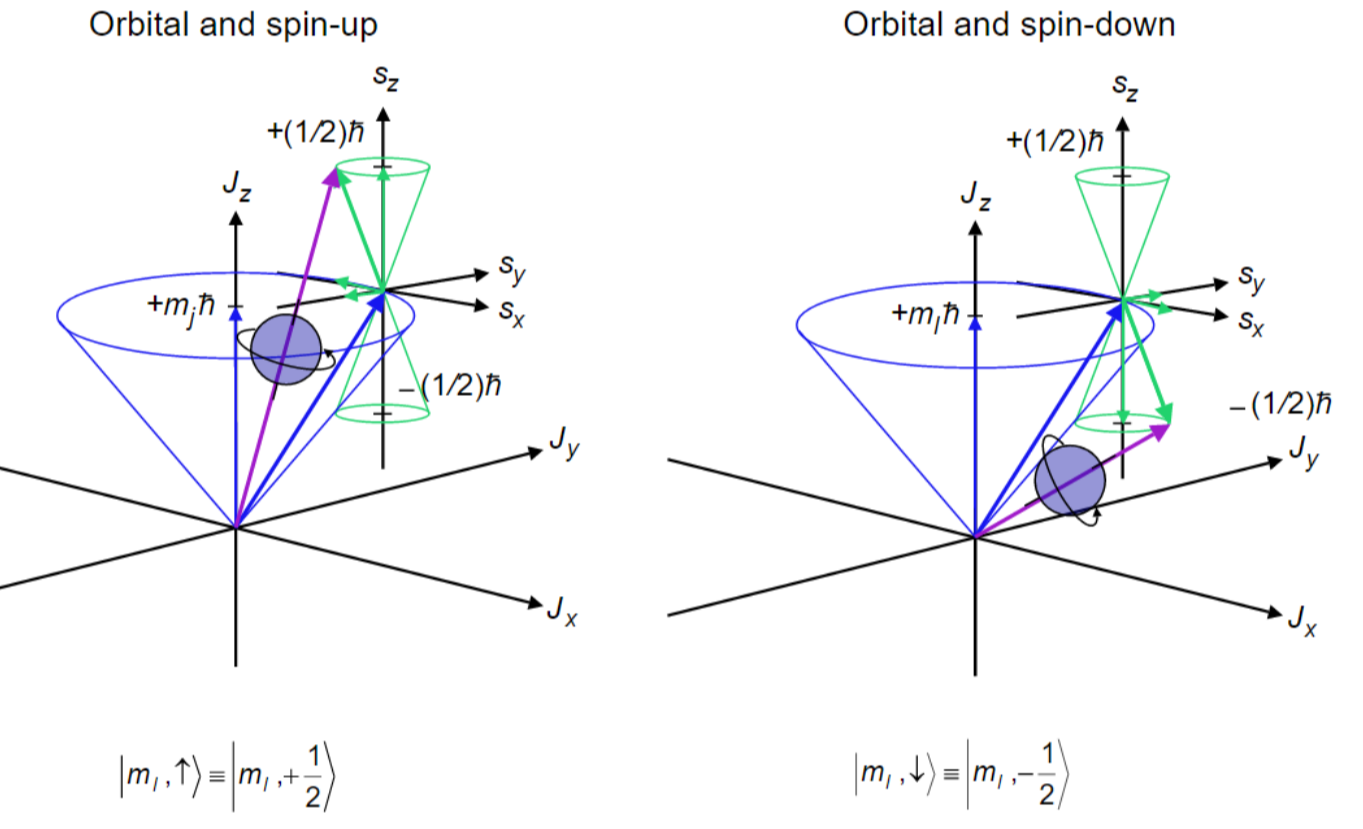
\includegraphics[width = .75\textwidth]{total_angular_momentum_visualized.png}
    \caption{Total angular momentum visualized in 3D.}
    \label{fig: total_angular_momentum_visualized}
    \end{figure}
\end{itemize}

\subsubsection{Total Angular Momentum of the Nucleus}
\begin{itemize}
    \item The sum of the angular momentum of all the nucleons in the nucleus. 
    \begin{align}
    \vec{I} &= \sum_{i=1}^{A} \vec{j}_i \quad , \quad  \vec{j}_i = \vec{l}_i + \vec{s}_i \\
    I &= \sqrt{I(I+1)}ℏ \\
    I_z &= mℏ \quad , \quad m ∈ \{-I, -I+1, \ldots, I-1, I\}
    \end{align} 
    \item As each nucleus has half-integer total angular momentum, odd number of nucleons $A$ will have half-integer total angular momentum, and even number of nucleons will have integer total angular momentum.
    \item All the known even-even nuclei have spin-0 ground states. 
    \item As a result, the ground state of an odd $A$ nucleus must be the $j$-value of the odd proton or neutron. 
\end{itemize}

\subsection{Parity}
Parity is the behavior of a system under the inversion of all spatial coordinates $\vec{r} → - \vec{r}$
\begin{itemize}
    \item Cartesian coordinates: $r → (-x, -y, -z)$. 
    \item Spherical coordinates: $r → (-r, π-θ, φ + π)$.
    \item The parity operator is $\hat{P}$ and has two effects on the wave function: 
    \begin{itemize}
        \item Even parity (+): $\hat{P}ψ(\vec{r}) = ψ(\vec{r})$.
        \item Odd parity (-): $\hat{P}ψ(\vec{r}) = -ψ(\vec{r})$.
        \item An even function is symmetric around the origin and an odd function is antisymmetric around the origin. This means $ψ(-r) = ψ(r)$ or $ψ(-r) = -ψ(r)$. 
        \item Visual representation \cref{fig: even_vs_odd_function}:
        \begin{figure}[h!]
        \centering
        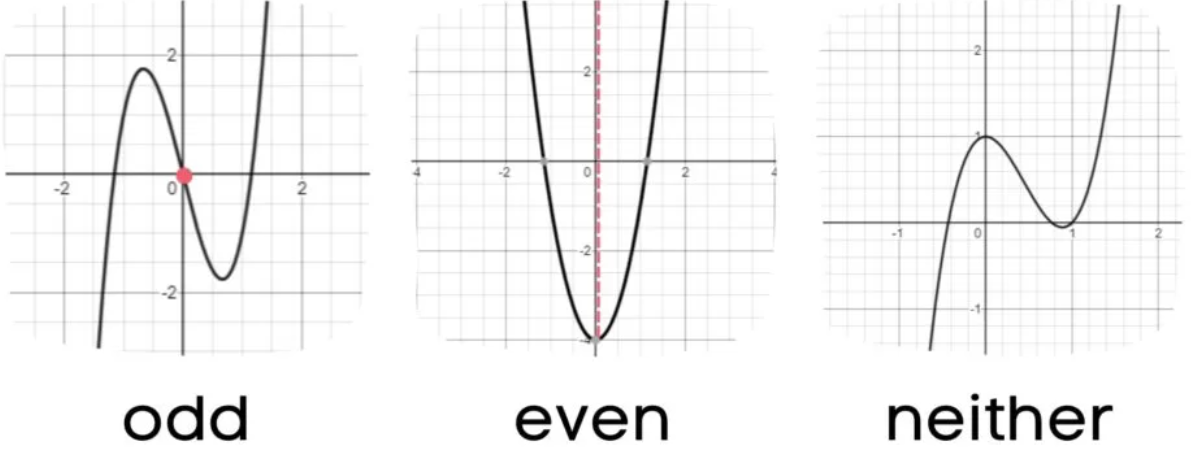
\includegraphics[width = .75\textwidth]{even_vs_odd_function.png}
        \caption{Visual representation of even and odd functions.}
        \label{fig: even_vs_odd_function}
        \end{figure}
    \end{itemize} 
\end{itemize}
\subsubsection{Splitting the Wave Function}
\begin{itemize}
    \item The wave function can be split into its radial and angular parts.
    \begin{align}
    Ψ(\vec{r}) &= R(r)Y(\theta, φ) \\
    \hat{P}R(r) &= R(r) \\
    \hat{P}Y(\theta, φ) &= (-1)^lY_{l}^{m}(θ, ϕ)
    \end{align} 
    \item Parity of state with orbital angular momentum $l$ 
    \begin{equation}
    π(-1)^{l}
    \end{equation} 
    \item By convention, the intrinsic parity of the nucleon is $π = +1$, because they are fermions. Anti-fermions (like positron) have $π = -1$.
    \item For a composite system, the parity is the product of the intrinsic parities of the constituents.
    \begin{equation}
      π_{\text{total}} = (-1)^{L}π_1π_2π_3 \ldots \quad , \quad  L = l_1 + l_2 + l_3 + \ldots
    \end{equation}
\end{itemize}

\section{Electric and Magnetic Moments}
\begin{itemize}
    \item The protons create a magnetic and electric fields. 
    \item A distribution of charge is assigned an electric dipole moment of either monopole, dipole, quadrupole, octopole, etc.
    \item A spherical charge distribution gives only a monopole. 
    \item A circular current only gives a magnetic dipole. 
    \item Nuclei tend to have as simple of dipole moments as possible. 
    \begin{itemize}
        \item L = 0: Monopole
        \item L = 1: Dipole
        \item L = 2: Quadrupole
        \item L = 3: Octopole
    \end{itemize}
\end{itemize}

\subsection{Parity Selection Rules}
\subsubsection\protect{Electric Dipole Moments $E_0$}
\begin{equation}
  L = 0, 2
\end{equation}
Allowed values are $L ∈ {0,2}$ with a parity of $(-1)^{L}$. A dipole is a measure of the separation of positive and negative charge. In the nucleus there is no separation. 

The electric monopole moment is just the charge of the nucleus $Z ⋅ e$.


\subsubsection\protect{Magnetic Dipole Moments $M_1$}
\begin{equation}
  L = 1
\end{equation}
Allowed values are $L = 1$ with a parity of $(-1)^{L+1} = 1$. The magnetic monopole has not been observed. 

As the charged particles are moving, they create a magnetic field. For an electron orbiting a nucleus, we get the following:
\begin{equation}
  \left|\vec{μ}\right| = \frac{e}{2πr / v} πr^2 = \frac{e}{2m}\left|\vec{l}\right|
\end{equation}
This connects the magnetic moment to the mass of the particle. The same goes for the protons in the nucleus. We know the $z$-component of the orbital angular momentum and can be inserted to the equation:
\begin{equation}
  μ = \frac{eℏ}{2m}l
\end{equation}
\subsection{Bohr Magneton \& Nuclear Magneton}
For atomic motion, the electron mass is used.
\begin{align}
μ_{B} = \frac{eℏ}{2m_{e}}  = 5.788 ⋅ 10^{-5} \text{ eV/T}
\end{align}
For nuclear motion, the proton mass is used.
\begin{align}
μ_{N} = \frac{eℏ}{2m_{p}}  = 3.152 ⋅ 10^{-8} \text{ eV/T}
\end{align}

As $μ_{B} ≫ μ_{N}$, the nuclear magnetic moment plays much smaller role in atomic physics.

\subsection{Magnetic Moments of Nuclei}
\begin{itemize}
    \item Magnetic Dipole Moment:
    \begin{itemize}
        \item The magnetic dipole moment of the nucleons is caused by their orbital motion. $μ = g_l μ_{N}l$. 
        \item The g-factor $g_l$ is a dimensionless quantity characterizing the magnetic moment of the atom, nucleus or other particle in question. 
        \item Protons have $g_l = 1$
        \item Neutrons have $g_l = -0.5$. It was believed to be zero, but it proves it's not a point particle.
    \end{itemize}
    \item Spin Magnetic Dipole Moment:
    \begin{itemize}
        \item The magnetic dipole moment of the nucleons is caused by their spin. $μ = g_s μ_{N}s$.
        \item The g-factor $g_s$ is a dimensionless quantity characterizing the magnetic moment of the atom, nucleus or other particle in question.
        \item Protons have $g_s = 5.59 ± 0.0000022$
        \item Neutrons have $g_s = -3.82 ± 0.0000022$. This is unexpected as the neutron is a neutral particle. This shows there charge inside the neutron, and it is not a point particle.
        \item Electrons have $g_s = 2$
    \end{itemize}
\end{itemize}

\subsubsection{Nuclear Structure from Magnetic Moments}
\begin{itemize}
    \item The pairing force favors the coupling of the nucleons such that the sum of their total angular momentum is zero. 
    \item As a result, the magnetic moment of the nucleus is determined by the unpaired nucleons.
    \item Example \cref{fig: nuclear_magnetic_dipole_samples}:
    \begin{figure}[h!]
    \centering
    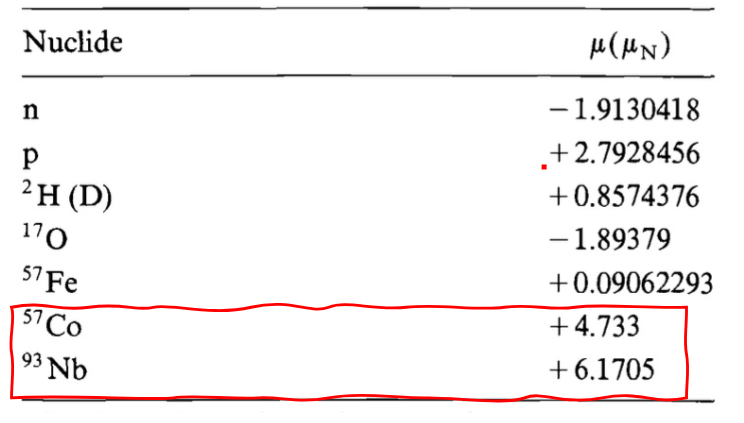
\includegraphics[width = .75\textwidth]{nuclear_magnetic_dipole_samples.png}
    \caption{Table showing the magnetic dipole moments of different nuclei. The box in red shows how larger atoms have a larger magnetic dipole moment, caused by more unpaired nucleons.}
    \label{fig: nuclear_magnetic_dipole_samples}
    \end{figure}
    
\end{itemize}

\subsection\protect{Electric Quadrupole Moments $E_2$ \& Shape of the Nucleus}
Visual representation of the electric quadrupole moments effect on the shape of the nucleus in \cref{fig: nucleus_shape_E2}. 
\begin{equation}
  eQ = e ∫ ψ^{*}(3z^2 - r^2)ψ \ \mathrm{d}v
\end{equation}
Experiment shows that large nuclei like Barium, has a pear-like shape. 
\begin{figure}[h!]
\centering
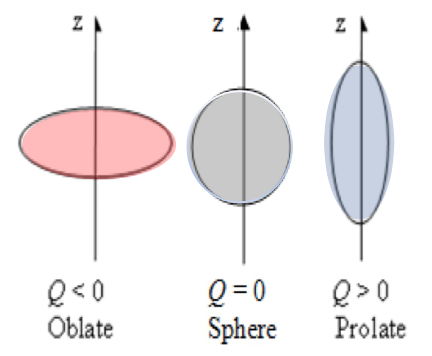
\includegraphics[width = .5\textwidth]{nucleus_shape_E2.png}
\caption{Shape of the nucleus as a function of the electric quadrupole moment.}
\label{fig: nucleus_shape_E2}
\end{figure}

\subsection{Example: Calculating Parity of State}
\paragraph{Case 1: Calculate the parity of two nucleons in the $p_{3 /2}$ orbital} 
In the $p_{3 /2}$ orbital, we know $l = 1$. As all nucleons are fermions, the parity $π$ of the orbital is $(-1)^l = -1$.
\paragraph{Case 2: Calculate the parity of two nucleons in the $g_{9 /2}$ orbital}
In the $g_{9 /2}$ orbital, we know $l = 4$. As all nucleons are fermions, the parity $π$ of the orbital is $(-1)^l = 1$.

\subsection{Level Schemes \& Excited States}
\begin{itemize}
    \item Some nuclei have more excited states than others. This is regularly associated with even-$Z$ and even-$N$ nuclei in the interval $150 ≤ A ≤ 190$. 
    \item Comparing the level schemes of different nuclei : 
    \begin{figure}[h!]
    \centering
    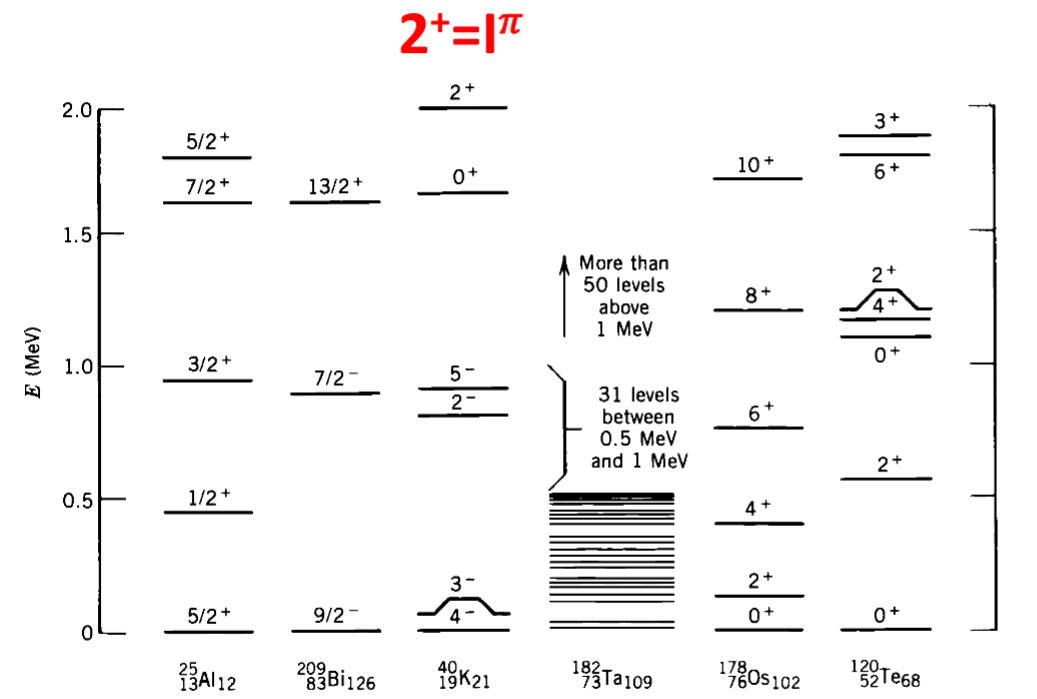
\includegraphics[width = .75\textwidth]{nuclei_excitation_levels_comparison.png}
    \caption{Some nuclei have more complex level schemes than others}
    \label{fig: nuclei_excitation_levels_comparison}
    \end{figure}
    
\end{itemize}


\section{Nuclear Force}
\begin{itemize}
    \item The strong force is very attractive at short distances. Even stronger than the Coulomb force. 
    \item Negligible at greater distances than 1-2 fm. 
    \item Some particles are immune, such as electrons. Electrons are 100,000 fm away from the nucleus.  
    \item The strong force becomes very repelling at distances smaller than 1 fm. 
    \item Nuclear force is nearly charge independent. We know this from experiments on excited states of \textit{mirror nuclei} (same $A$, but opposite $N$ and $Z$) as seen in \cref{fig: mirror_nuclei_excitation_levels_comparison}.
    \begin{figure}[h!]
    \centering
    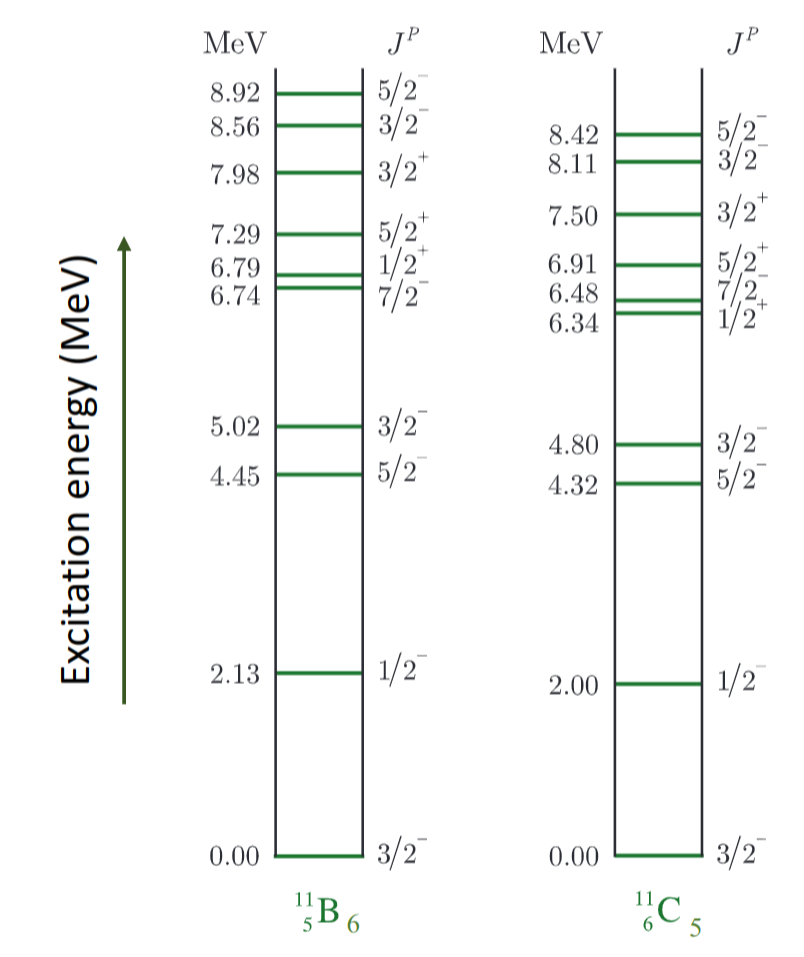
\includegraphics[width = .5\textwidth]{mirror_nuclei_excitation_levels_comparison.png}
    \caption{Comparison of the excitation levels of mirror nuclei. In this case we have $\displaystyle _{5}^{11}\text{B}_{6}$ and $\displaystyle _{6}^{11}\text{C}_{5}$}
    \label{fig: mirror_nuclei_excitation_levels_comparison}
    \end{figure} 
    
\end{itemize}

\subsection{Effects of the Short Range of the Strong Force}
\begin{itemize}
    \item When shooting alpha particles at a nucleus, the alpha particles are repelled by the Coulomb force if they do not have enough energy to get close enough to the nucleus. Then the strong force takes over and the alpha particles are attracted to the nucleus. This is why the Rutherford model does not work at lower energies. 
    \item The linear dependence on the binding energy per nucleon shows that the strong force is short range. If it were long range, each nucleon would attract all the others. Then the term in the binding energy as seen in the first therm of \cref{eq: semi_empirical_mass_formula}, would be quadratic and not linear $(α_vA)$
\end{itemize}

\subsection{Deuteron}
\begin{itemize}
    \item Consist of a proton and a neutron (nucleus of deuterium).
    \item To understand the structure of the atoms we would need to study its excited states. The problem is that deuteron is weakly bound and has no excited states.
\end{itemize}
\subsubsection{Deuteron Binding Energy}
There are multiple ways of calculating the binding energy of the deuteron. 
\begin{enumerate}
    \item \textbf{Mass spectroscopy}: Find the difference in mass between the deuteron and the proton and neutron.
    \begin{equation}
      B = \left( M\left(_{}^{1}\text{H}_{}\right) + m_n - m\left(_{}^{2}\text{H}_{}\right)\right)c^2 = 2.225 \text{ MeV}
    \end{equation} 
    \item \textbf{Nuclear reaction}: The gamma ray emitted when a neutron is captured by a proton is almost the binding energy. It has only energy, but can be converted to mass through $E = mc^2$.
    \begin{align}
    _{}^{1}\text{H}_{}& + n → \ce{_{}^{2}\text{H}_{}} + γ \\ 
    E_{γ} &≈ B = M_{\text{initial}} - M_{\text{final}} \\
    B &= \left( M\left(_{}^{1}\text{H}_{}\right) + m_n - M\left(_{}^{2}\text{H}_{}\right)\right)c^2 = 2.224 \text{ MeV}
    \end{align}
\end{enumerate}

\subsubsection{Nucleon-Nucleon Potential}
\begin{itemize}
    \item We assume that the potential between the nucleons is a finite square well with a potential depth of $-V_0$
    \item Solving for the Schrödinger equation for specific energy values and applying the boundary conditions we get the following results:
    \begin{align}
    &k_1 \cot \left(k_1 \vec{R}\right) = -k_2 \\
    &k_1 = \sqrt{\frac{2mE}{\hbar^2}} \quad k_2 = \sqrt{\frac{2m\left(V_0 + E\right)}{\hbar^2}}
    \end{align}
    \item The radius $R$ is now connected to the energy, and we know from scattering experiments that the radius is around 2.1 fm.
    \item The solution gives a potential of $V_0 = 35$ MeV. 
    \item The binding energy of the deuteron is just below the potential depth as seen in \cref{fig: deuteron_potential}.
    \begin{figure}[h!]
    \centering
    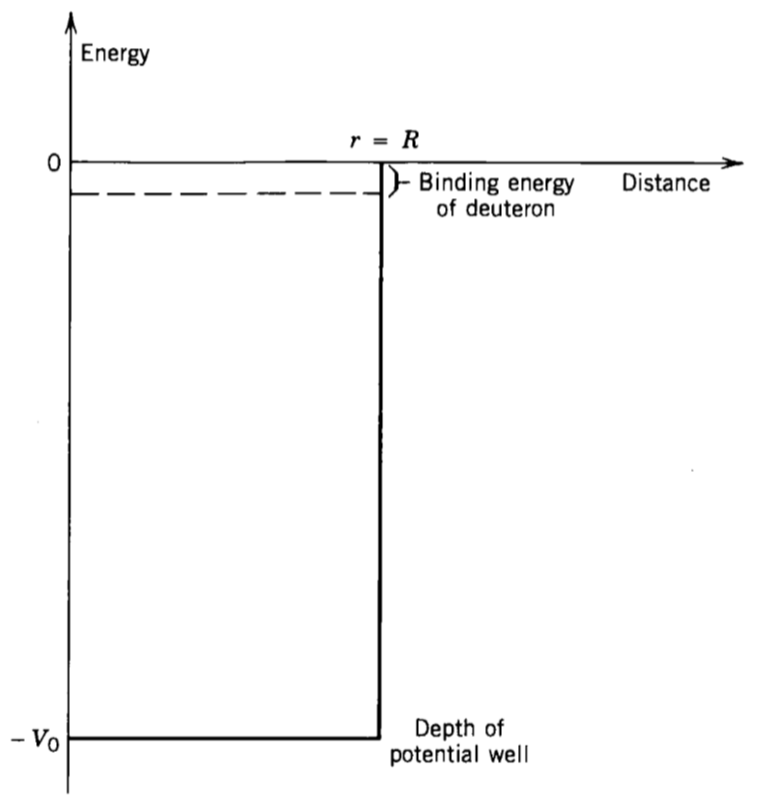
\includegraphics[width = .5\textwidth]{deuteron_potential.png}
    \caption{Square well potential for the deuteron. }
    \label{fig: deuteron_potential}
    \end{figure}
\end{itemize}

\subsubsection{Deuteron Spin and Parity}
\paragraph{Total Spin:}
\begin{equation}
  \vec{I} = \vec{S}_p + \vec{S}_n + \vec{l}
\end{equation}
\paragraph{Spin Configuration with $I = 1$}
\begin{enumerate}
    \item Aligning the spins gives $I = 1$ and $S = 1$ with $l = 0$. This is a positive parity state with $π = (-1)^{l} = 1$. We then get $I^{π}$ 
    \item Aligning the spins with gives $I = 3$
\end{enumerate}

\paragraph{Electric Quadrupole Moment}
The deuteron has a small non-zero electric quadrupole moment. This makes it so about 4\% of the time the deuteron is in an excited state with $l = 2$. \section{The Standard Model}
\begin{itemize}
    \item The periodic table of particle physics.
    \item Categorized as seen in \cref{fig: SM_particles}.
\end{itemize}

\subsection{The Particles}
\begin{itemize}
    \item \textbf{Quarks}: 
    \begin{itemize}
        \item Each quark pair from each generation has one up-type and one down-type quark. The up-type quarks have a charge of $+\frac{2}{3}e$, and the down-type quarks have a charge of $-\frac{1}{3}e$. 
        \item The quarks are bound together by the strong force, mediated by the gluons. 
        \item They are all spin-half particles.
        \item They can interact through the weak force, electromagnetic force, and the strong force.
        \item Each quark is considered a quark flavor.
    \end{itemize}
    \item \textbf{Leptons}:
    \begin{itemize}
        \item The leptons are divided into three generations, each with a charged lepton and a neutrino.
        \item The charged leptons all have a charge of $-e$, and the neutrinos are neutral.
        \item They all have half-integer spin.
        \item The charged leptons are much lighter than the neutrinos. 
        \item The charged leptons interact with the weak force and the electromagnetic force, while the neutrinos only interact with the weak force.
        \item Each lepton is considered a lepton flavor.
    \end{itemize}
    \item \textbf{Bosons}:
    \item \textbf{Fermions}: All quarks and leptons are fermions, which means they have half-integer spin.
    \item \textbf{Higgs Boson}: Gives mass to all the particles. Can interact with itself, as it has mass. 
\end{itemize}

\subsection{The Forces}
\begin{itemize}
    \item \textbf{Electromagnetic Force}: 
    \begin{itemize}
        \item Mediated by the photon.
        \item Acts between particles with electric charge.
    \end{itemize} 
    \item \textbf{Weak Force}: 
    \begin{itemize}
        \item Mediated by the $W^{\pm}$ and $Z^0$ bosons.
        \item The $W^{±}$ has electric charge and can interact with itself and other particles with electric charge.
        \item 
    \end{itemize}
    \item \textbf{Strong Force}: 
    \begin{itemize}
        \item Mediated by gluons with strong force charge. 
        \item  The gluon has a strong force charge, making it able to interact with itself. 
    \end{itemize}
\end{itemize}

\begin{figure}[h!]
\centering
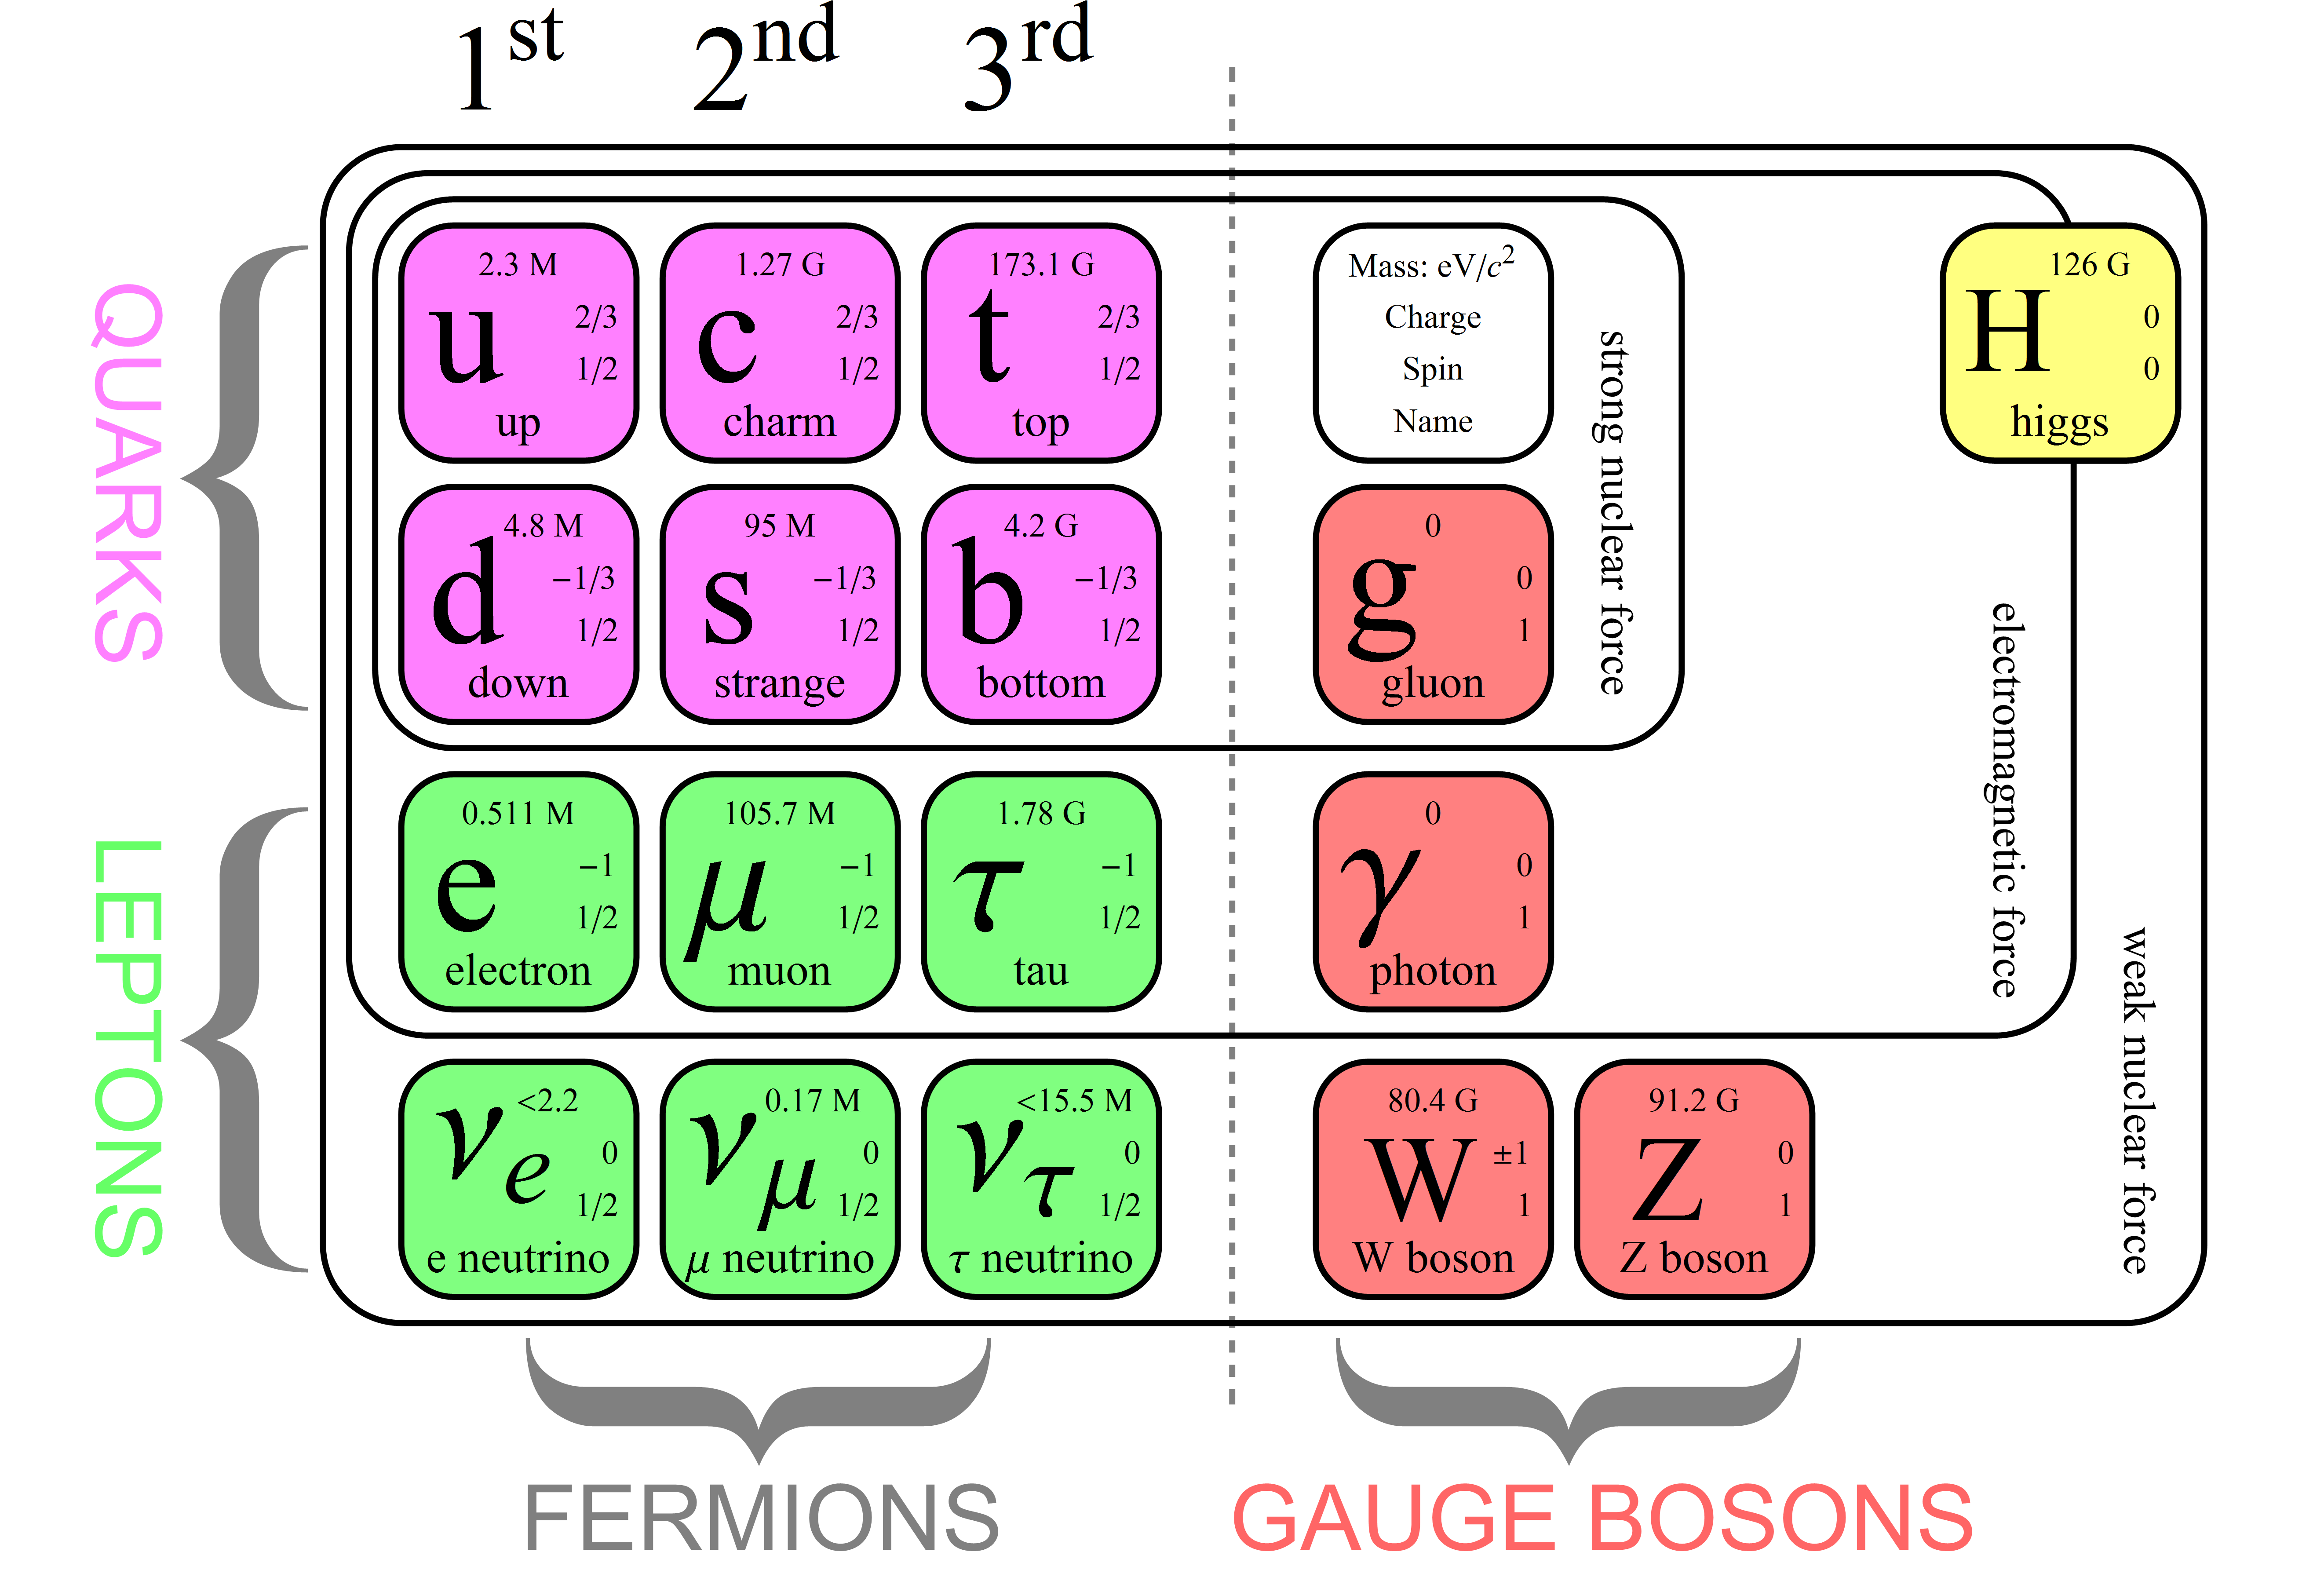
\includegraphics[width = .9\textwidth]{SM_particles.png}
\caption{Figure showing the particles of the Standard Model, and their respective forces. Each column represents a generation of particles.}
\label{fig: SM_particles}
\end{figure}


\section{Feynman Diagrams}
\begin{itemize}
    \item A graphical representation of particle interactions.
    \item Time goes from left to right.
    \item The particles are represented by lines, and the interactions are represented by vertices.
    \item \textbf{Fermions}: 
    \begin{itemize}
        \item Represented by straight lines with arrows
        \item Anti-particles are represented by straight lines with arrows pointing in the opposite direction.
    \end{itemize}
    \item \textbf{Electromagnetic/Weak Interactions}:
    \begin{itemize}
        \item Represented by wavy lines
        \item Virtual photons (often noted by an asterisk) may have mass and may not move at the speed of light
    \end{itemize}
    \item \textbf{Strong Interactions}: Represented by curly lines.
    \item \textbf{Higgs Boson}: Represented by a dashed line.
\end{itemize}

\subsection{Allowed Vertices (\cref{fig: feynman_diagram_vertices})}
\begin{figure}[h!]
\centering
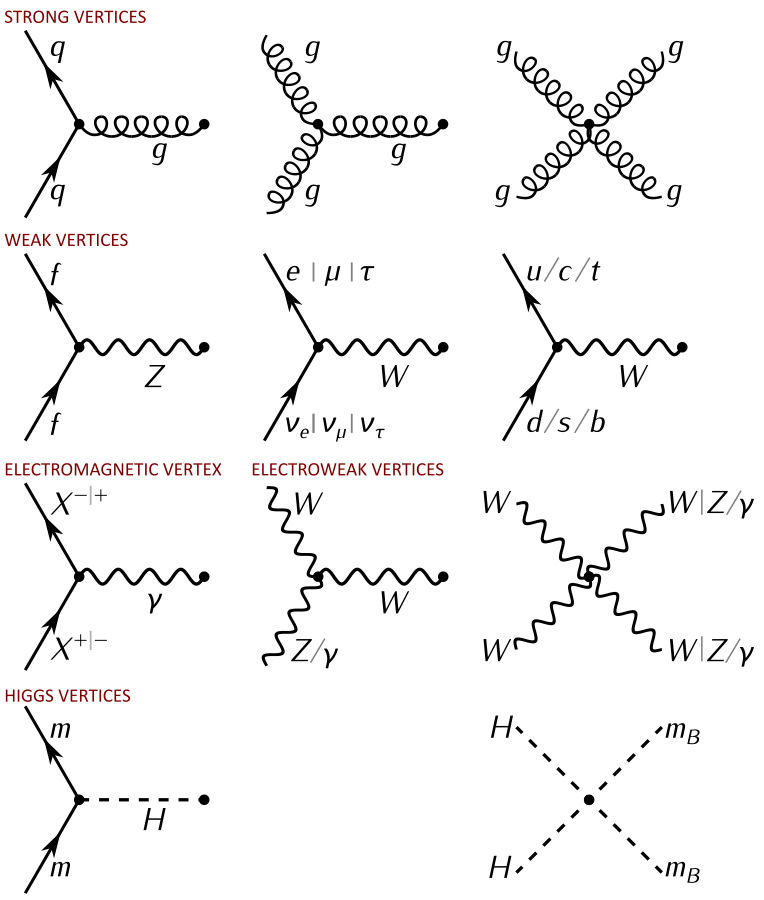
\includegraphics[width = \textwidth]{feynman_diagram_vertices.png}
\caption{Figure of all allowed vertices in the Standard Model.}
\label{fig: feynman_diagram_vertices}
\end{figure}
% \subsection{Charges}
% \begin{itemize}
%     \item The charges are $α_{\text{W}}, α_{\text{W}}, α_{\text{S}}$, for the weak, electromagnetic, and strong force, respectively.
%     \item The product of the charges show how likely an interaction is to happen.
% \end{itemize}


test 
test
\end{document}
